\documentclass[]{beamer}
\usepackage[utf8]{inputenc}
\usepackage{xparse}
\usepackage{microtype}
\usepackage{graphicx}
\usepackage{amsmath}
\usepackage{amsthm}
\usepackage{amsfonts}
\usepackage{listings}
\usepackage{bbm}
\usepackage{placeins}
\usepackage{tikz}
\usepackage{algorithm}
\usepackage{xcolor}
\usepackage{algpseudocode}
\usepackage[
    %backend=biber,
    natbib=true,
    style=numeric,
    sorting=none
]{biblatex}
\usepackage{pgfplots}
\pgfplotsset{compat=1.10}
\usepgfplotslibrary{fillbetween}
\addbibresource{bib.bib}

\usetheme{metropolis}
\title{Optimization-inspired Barriers in Nested Sampling}
\date{\today}
\author{Farin Lippmann}
\institute{Friedrich-Schiller-University Jena \\\\ Supervisor: Prof. Dr. Michael Habeck}
\date{13.01.2025}
\begin{document}
  \maketitle
  \begin{frame}{Table of Contents}
    \tableofcontents
  \end{frame}
  \section{Background}
  \subsection*{Nested Sampling}
  \begin{frame}{Nested Sampling - Overview}
    Introduced by Skilling \cite{skilling}.

    Input:
    \begin{itemize}
      \item likelihood and
      \item prior of a parameterized generative statistical model
      \item data from the process that is being modeled
    \end{itemize}
    Output:
    \begin{itemize}
      \item samples from the posterior distribution of parameter values
      \item an estimate of the evidence (useful for model comparison)
    \end{itemize}
  \end{frame}
  \begin{frame}{Nested Sampling - Bayes' Theorem}
    \centering
    \scalebox{1.5}{
      $
        \overbrace{P(\theta \, | \, D)}^{\textnormal{Posterior}} = \frac{\overbrace{P(D \,|\, \theta)}^{\textnormal{Likelihood}} \; \overbrace{P(\theta)}^{\textnormal{Prior}}}{\underbrace{P(D)}_{\textnormal{Evidence}}} = \frac{L(\theta) \; \pi(\theta)}{ Z }
      $
    }
  \end{frame}
  \begin{frame}{Nested Sampling - Algorithm}
    \begin{itemize}
      \item generate samples iteratively and slowly raise a minimum likelihood samples must satisfy
      \item use an ensemble of points (``live points'') $\theta_1 ... \, \theta_n$
      \item in each iteration:
        \begin{itemize}
          \item remove the lowest-likelihood point $\theta_{\textnormal{min}}$
          \item estimate its contribution to the evidence
          \item set $L^* \leftarrow L(\theta_{\textnormal{min}})$ as the new likelihood constraint
          \item sample a new point from the constrained prior $\theta_{\textnormal{new}} \sim \pi(\theta) \mathbbm{1}_{\{L(\theta) > L^*\}}(\theta)$ and add it to the live points
        \end{itemize}
      \item repeat until some stopping criteria are fulfilled
    \end{itemize}
  \end{frame}
  \begin{frame}{Nested Sampling - A Visualization}
    \centering
    \includegraphics[trim={3.4cm 1.3cm 3.2cm 1.4cm}, clip, width=0.45\textwidth]{figs/ns_eggcrate_example_1.png}
    \includegraphics[trim={3.4cm 1.3cm 3.2cm 1.4cm}, clip, width=0.45\textwidth]{figs/ns_eggcrate_example_2.png}
  \end{frame}

  \begin{frame}{Nested Sampling - Likelihood-Restricted Prior Sampling}
    Sampling from the constrained prior $\theta_{\textnormal{new}} \sim \pi(\theta) \mathbbm{1}_{\{L(\theta) > L^*\}}(\theta)$
    
    Skilling: ``such points will usually be found by some MCMC approximation, ...'' \cite[6]{skilling}
    \vspace{0.3cm}

    \centering
    \begin{minipage}{0.45\textwidth}
      \centering
      \textbf{Metropolis-Hastings}
      \vspace{0.5cm}
      \includegraphics[trim={1.5cm, 1.3cm, 1.1cm, 1.5cm}, clip, scale=0.4]{figs/metropolis_example.png}
    \end{minipage}
    \begin{minipage}{0.45\textwidth}
      \centering
      \textbf{Hamiltonian Monte Carlo}
      \vspace{0.5cm}
      \includegraphics[scale=0.4]{figs/hmc_example.png}
    \end{minipage}
  \end{frame}

  \subsection*{The Barrier Method}
  \begin{frame}{The Barrier Method - The Problem}
    Solves optimization problems of the form
    \begin{align*}
      &\textnormal{minimize} && f(x) && \\
      &\textnormal{subject to}  && f_i(x) \leq 0 \quad \textnormal{for} \; i=1,...,m &&
    \end{align*}
    with $f$ and all $f_i$ being convex and twice continuously differentiable \cite[561]{boyd}.
  \end{frame}
  \begin{frame}{The Barrier Method - Exact Barriers}
    Incorporate constraints into the objective function:
    \begin{align*}
      &\textrm{minimize} && f(x) + \sum_{i=1}^m \mathcal{I}(f_i(x))&&
    \end{align*}
    with:
    \begin{equation*}
      \mathcal{I}(u) = \begin{cases}
            0,      & \text{if }  u \leq 0\\
            \infty, & \text{if }  u > 0
            \end{cases}
    \end{equation*}
    
    Accurately represents the problem, but is not differentiable.
  \end{frame}
  \begin{frame}{The Barrier Method - Log Barriers}
    Log barrier function:
    \begin{align*}
      \hat{\mathcal{I}}(u)= -\frac{1}{t}\log(-u)
    \end{align*}
    with parameter $t$.

    \begin{center}
    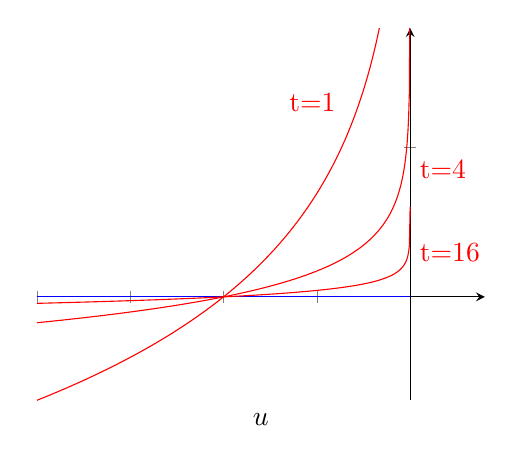
\begin{tikzpicture}
      \begin{axis} [
          axis lines=center,
          xticklabel=\empty,
          yticklabel=\empty,
          xlabel=$u$,
          x label style={at={(axis description cs:0.5,-0.01)},anchor=north},
          ymax=1.8,
          xmax=0.4,
          scale=0.83
      ]
      \addplot[
          domain=-2:0, 
          samples=100,
          color=blue,
          line width=0.1mm
      ] { 0 };
      \addplot[
          domain=-2:0, 
          samples=500,
          color=red
      ] { -(1/1)*ln(-x) };
      \addplot[
          domain=-2:0, 
          samples=500,
          color=red
      ] { -(1/4)*ln(-x) };
      \addplot[
          domain=-2:0, 
          samples=500,
          color=red
      ] { -(1/16)*ln(-x) };
      \node[color=red, anchor=west] at (axis cs: -0.7, 1.3) {t=1};
      \node[color=red, anchor=west] at (axis cs: 0, 0.85) {t=4};
      \node[color=red, anchor=west] at (axis cs: 0, 0.3) {t=16};
      \end{axis}
    \end{tikzpicture}
    \end{center}
  \end{frame}
  \begin{frame}{The Barrier Method - Approximate Optimization Problem}
    \begin{align*}
      &\textrm{minimize} && f(x) + \sum_{i=1}^m -\frac{1}{t}\log(-f_i(x))&&
    \end{align*}
    \pause
    Multiply objective function by $t$ to obtain:
    \begin{align*}
      &\textrm{minimize} && t \cdot f(x) + \sum_{i=1}^m -\log(-f_i(x))&&
    \end{align*}
    There is a different solution $x^*(t)$ for each value of $t$. 
    As $t \rightarrow \infty$, $x^*(t)$ approaches the real solution \cite[p. 561ff.]{boyd}.
  \end{frame}

  \begin{frame}{The Barrier Method - Central Path}
    \centering
    \includegraphics[trim={1.4cm 0.8cm 1cm 0.8cm}, clip, scale=0.6]{figs/barrier_method_example.png}
  \end{frame}

  \begin{frame}{The Barrier Method - The Idea}
    $x^*(t)$ for a high value of $t$ is a good estimation, but has extreme derivatives.

    \pause
    Stabilize by using a good starting point, a solution using a lower value of $t$. $\rightarrow$ Bootstrapping.
  \end{frame}

  \section{Nested Sampling with Barriers}
  \subsection{Motivation}
  \begin{frame}{Nested Sampling with Barriers - Motivation}
    \begin{itemize}
      \item LRPS is difficult \pause
      \item Ratio of the valid area to the area of the whole sample space decreases steadily, finding samples becomes harder. \pause
      \item Result: low acceptance rates or (if using an adaptive step size) highly correlated samples. \pause
      \item These methods only notice the likelihood constraint boundary once they cross it. \pause
      \item $\implies$ Would like an approach that feels the boundary earlier and pushes the samples away from it. \pause
      \item The log barrier lends itself to this idea.
    \end{itemize}
  \end{frame}
  \subsection{Derivation}
  \begin{frame}{Derivation - Pretend Optimization}
    We pretend that likelihood-restricted prior sampling (LRPS) is an optimization problem.
    \begin{eqnarray*}
      \quad &\textrm{maximize} \quad\quad\quad \pi(\theta) \quad &\textrm{subject to} \quad L(\theta) > L^* \\ \pause
      \iff \; &\textrm{minimize} \quad -\log(\pi(\theta)) &\textrm{subject to} \quad l(\theta) > l^* \\ \pause
      \iff \; &\textrm{minimize} \quad -\log(\pi(\theta)) &\textrm{subject to} \quad l^* - l(\theta) < 0
    \end{eqnarray*}
    Incorporate constraints into objective function:
    $$
      \textrm{minimize} \quad -\log(\pi(\theta)) + \mathcal{I}(l^* - l(\theta))
    $$
  \end{frame}
  \begin{frame}{Derivation - The Log Barrier Term}
    Associated approximate problem using log barriers:
    \begin{align*}
      &\textrm{minimize} \quad -\log(\pi(\theta)) + \hat{\mathcal{I}}(l^* - l(\theta)) \\
      \iff \; &\textrm{minimize} \quad -\log(\pi(\theta)) - \frac{1}{t}\log(l(\theta) - l^*)
    \end{align*}
    \pause
    Negate and exponentiate to return to a maximization problem in probability space:
    \begin{align*}
      &\textrm{maximize} \quad \exp\left(-\left(-\log(\pi(\theta)) - \frac{1}{t}\log(l(\theta) - l^*)\right)\right) \\
      \iff \; &\textrm{maximize} \quad \pi(\theta) \, (l(\theta) - l^*)^{\frac{1}{t}}
    \end{align*}
  \end{frame}
  \begin{frame}{Derivation - Introducing $q$}
    Expand sampling space:
    $$
      \theta \rightarrow (\theta, q)
    $$
    \pause
    Start by assuming independence:
    $$
      P(\theta, q) = P(\theta) \, P(q)
    $$
    \pause
    This independence follows through to the likelihood, prior and evidence:
    \begin{align*}
      L(\theta, q) &= L_\theta(\theta) \, L_q(q) \\
      \pi(\theta, q) &= \pi_\theta(\theta) \, \pi_q(q) \\
      Z_{\theta, q} &= Z_{\theta} \, Z_q
    \end{align*}
  \end{frame}
  \begin{frame}{Derivation - LRPS on the Expanded Space}
    Likelihood-restricted prior sampling on the expanded space:
    \begin{align*}
      (\theta,q) \sim \; &\bar{\pi}(\theta, q \,|\, L^*) \\
      &\bar{\pi}(\theta, q \,|\, L^*) = \pi(\theta, q) \, \mathbbm{1}_{\{L(\theta, q) \, > \, L^*\}}(\theta, q)
    \end{align*}
    \pause
    Use collapsed Gibbs sampling \cite{collapsed_gibbs}:
    \begin{align*}
      \theta &\sim  \bar{\pi}(\theta \,|\, L^*) \\
      q &\sim  \bar{\pi}(q \,|\, L^*, \theta)
    \end{align*}
  \end{frame}
  \begin{frame}{Derivation - LRPS on the Expanded Space}
    Define: 
    $$
      L_q(q) = \frac{1}{q}
    $$
    \pause
    Now we can reshape the likelihood-restricted priors:
    \begin{align*}
      \bar{\pi}(\theta \,|\, L^*) &= \int_{q_{\textrm{min}}}^{q_{\textrm{max}}} \bar{\pi}(\theta, q \,|\, L^*) \; dq \\
      &= \int_{q_{\textrm{min}}}^{q_{\textrm{max}}} \pi_\theta(\theta) \, \pi_q(q) \, \mathbbm{1}_{\{L(\theta, q) \,>\, L^*\}}(\theta, q) \; dq \\
      &= \pi_\theta(\theta) \int_{q_{\textrm{min}}}^{L^* / L_\theta(\theta)} \pi_q(q) \; dq \\
      &= \pi_\theta(\theta) \; \Pi_q(L_\theta(\theta) / L^*) \\
      \bar{\pi}(q \,|\, L^*, \theta) &= \pi_q(q) \, \mathbbm{1}_{\{q < L_\theta(\theta) / L^*\}}(q)
    \end{align*}
  \end{frame}
  \begin{frame}{Derivation - LRPS on the expanded Space}
    Add the log barrier term via the CDF of $q$:
    \begin{eqnarray*}
      \Pi_q(L_\theta(\theta) / L^*) && \overset{!}{=} \quad (l_\theta(\theta) - l^*)^{\frac{1}{t}}  \\\pause
      \Pi_q(L_\theta(\theta) / L^*) && = \quad \log(L_\theta(\theta) / L^*)^{\frac{1}{t}} \\\pause
      \textrm{let } q &&= L_\theta(\theta) / L^* \\\pause
      \Pi_q(q) &&= \log(q)^{\frac{1}{t}} 
    \end{eqnarray*}
    Also implicitly defined $q_{\textnormal{min}} = 1$.
  \end{frame}
  \begin{frame}{Derivation - Unnormalized CDF of $q$}
    \centering
    \begin{tikzpicture}
      \begin{axis} [
          axis lines=center,
          xlabel=$q$,
          x label style={at={(axis description cs:0.5,-0.1)},anchor=north},
          xmin=0,
          xmax=5,
          ymax=2
      ]
      \addplot[
          domain=1:10, 
          samples=500,
          color=red
      ] { ln(x)^(1/0.5) };
      \addplot[
          domain=1:10, 
          samples=500,
          color=blue
      ] { ln(x)^(1/1) };
      \addplot[
          domain=1:10, 
          samples=500,
          color=orange
      ] { ln(x)^(1/4) };
      \node[color=red, anchor=east] at (axis cs: 3.8, 1.9) {t=0.5};
      \node[color=blue, anchor=east] at (axis cs: 4.7, 1.6) {t=1};
      \node[color=orange, anchor=east] at (axis cs: 4.5, 1.0) {t=4};
      \end{axis}
    \end{tikzpicture}
  \end{frame}
  \begin{frame}{Derivation - Nested Sampling with Barriers}
    With likelihood and prior of $q$ defined and the log barrier term incorporated, we have a new algorithm.
    \pause

    Changes from the original Nested Sampling:
    \begin{enumerate}
      \item Set new parameters: $t > 0$ and $q_{\textnormal{max}} > 1$.\pause
      \item For each starting $\theta$, also sample a $q$.\pause
      \item Use the joint likelihoods of $\theta$ and $q$, $L(\theta, q) = \frac{L_\theta(\theta)}{q}$, instead of just the likelihood of $\theta$.\pause
      \item Sample $\theta_{\textnormal{new}}$ from the modified constrained prior $\pi_\theta(\theta) \, \Pi_q(l_\theta(\theta) - l^*)$.\pause
      \item Sample $q_{\textnormal{new}}$ from the constrained prior $\pi_q(q) \, \mathbbm{1}_{\{q < L_\theta(\theta_{\textnormal{new}}) / L^*\}}(q)$ dependent on the sampled $\theta_{\textnormal{new}}$.\pause
      \item Divide out $Z_q(t, q_{\textnormal{max}})$ from the evidence before returning it.
    \end{enumerate}
  \end{frame}
  \begin{frame}{Derivation - A Visualization}
    \centering
    LRPS using HMC in Nested Sampling with Barriers
    \includegraphics[trim={3.2cm, 1cm, 2.85cm, 1cm}, clip, scale=0.6]{figs/barrier_sampling_hmc.png}
  \end{frame}
  \subsection{Interpretation}
  \begin{frame}{Interpretation - $q$}
    \begin{itemize}
      \item Each $\theta$ is paired with a $q$. \pause
      \item $L(\theta, q) = \frac{L_\theta(\theta)}{q}$ and $q > 1$. \pause
      \item $\implies$ The likelihood of each $\theta$ is reduced by its $q$. \pause
      \item Since $Z_q$ is divided out, this only influences sampling. \pause
      \item $q$ is sampled from $\pi_q(q) \, \mathbbm{1}_{\{q < L_\theta(\theta) / L^*\}}(q)$ \pause
      \item $\implies$ $\theta$ further away from the constraint barrier tend to have higher $q$, reducing their likelihood \pause
      \item Interpretation: the lowered likelihood makes up for the log barrier term encouraging samples further away from the constraint \pause
      \item If the likelihoods were not lowered, the constraint would rise much more quickly than in standard Nested Sampling
    \end{itemize}
  \end{frame}
  \begin{frame}{Interpretation - $t$ and $q_{\textnormal{max}}$}
    \begin{itemize}
      \item $t$ and $q_{\textnormal{max}}$ influence the shape and support of $q$'s distribution \pause
      \item Since the log barrier term is incorporated using $q$'s CDF, they also influence how the log barrier term acts. \pause
      \item Larger $q_{\textnormal{max}}$ $\implies$ the log barrier term affects sampling earlier \pause
      \item Larger $t$ $\implies$ the log barrier becomes steeper, affecting only values closer to the boundary
    \end{itemize}
  \end{frame}
  \begin{frame}{Interpretation - $t$ and $q_{\textnormal{max}}$}
    \centering
      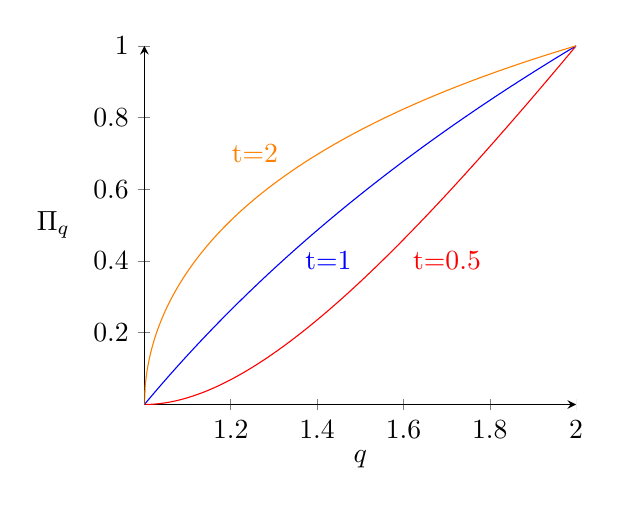
\begin{tikzpicture}
        \begin{axis} [
            axis lines=center,
            xlabel=$q$,
            x label style={at={(axis description cs:0.5,-0.1)},anchor=north},
            y label style={at={(axis description cs:-0.15, 0.5)},anchor=east},
            ylabel=$\Pi_q$,
            xmax=2,
            scale=0.8
        ]
        \addplot[
            domain=1:2, 
            samples=1000,
            color=red
        ] { ln(x)^(1/0.5) / (ln(2)^(1/0.5)) };
        \addplot[
            domain=1:2, 
            samples=500,
            color=blue
        ] { ln(x)^(1/1) / (ln(2)^(1/1)) };
        \addplot[
            domain=1:2, 
            samples=500,
            color=orange
        ] { ln(x)^(1/2) / (ln(2)^(1/2)) };
        \node[color=red, anchor=west] at (axis cs: 1.6, 0.4) {t=0.5};
        \node[color=blue, anchor=west] at (axis cs: 1.35, 0.4) {t=1};
        \node[color=orange, anchor=west] at (axis cs: 1.18, 0.7) {t=2};
        \end{axis}
      \end{tikzpicture}
  \end{frame}
  \section{Results}
  \subsection*{Setup}
  \begin{frame}{Setup - Example Problems}
    Gaussian mixtures with two components, one slab and a spike:
    \begin{itemize}
      \item $L_1(\theta) = 100 \, \mathcal{N}(\theta \,|\, \mu=0, \Sigma= u I_{20}) + \mathcal{N}(\theta \,|\, \mu=0, \Sigma= v I_{20})$
      \item $L_2(\theta) = 100 \, \mathcal{N}(\theta \,|\, \mu=(0.2, 0.2, ..., 0.2), \Sigma= u I_{20}) + \mathcal{N}(\theta \,|\, \mu=0, \Sigma= v I_{20})$
    \end{itemize}
    with $u = 0.01$ and $v = 0.1$.
  \end{frame}
  \begin{frame}{Setup - Configurations}
    These configurations were tested:
    \begin{itemize}
      \item Metropolis Algorithm (with simple adaptive step size)
      \item HMC with reflection (only for standard Nested Sampling, with simple adaptive step size) \cite{hmc_in_ns}
      \item HMC (only for Nested Sampling with Barriers, with simple adaptive step size)
      \item an optimal method for sampling inside a $d$-ball (only for the $L_1$-problem with Standard Nested Sampling; labeled ``Ball'' in the figures)  
    \end{itemize}
  \end{frame}
  \subsection*{Nested Sampling with and without Barriers}
  \begin{frame}{Nested Sampling with and without Barriers - Evidence Estimates}
    \centering
    \includegraphics[trim={2cm, 0cm, 1.8cm, 0cm}, clip, scale=0.6]{figs/results/logZ_diffs_spike_20d.png}
  \end{frame}
  \begin{frame}{Nested Sampling with and without Barriers - Evidence Estimates}
    \centering
    \includegraphics[trim={2cm, 0cm, 1.8cm, 0cm}, clip, scale=0.6]{figs/results/logZ_diffs_spike_offcenter_20d.png}
  \end{frame}
  \begin{frame}{Nested Sampling with and without Barriers - Posterior Modes Found}
    \centering
    \includegraphics[scale=0.52]{figs/results/modes_found_spike_20d.png}
  \end{frame}
  \begin{frame}{Nested Sampling with and without Barriers - Posterior Modes Found}
    \centering
    \includegraphics[scale=0.52]{figs/results/modes_found_spike_offcenter_20d.png}
  \end{frame}
  \begin{frame}{Nested Sampling with and without Barriers - Iterations}
    \centering
    \includegraphics[trim={0cm, 0cm, 1.8cm, 0cm}, clip, scale=0.6]{figs/results/iterations_spike_20d.png}
  \end{frame}
  \begin{frame}{Nested Sampling with and without Barriers - Iterations}
    \centering
    \includegraphics[trim={0cm, 0cm, 1.8cm, 0cm}, clip, scale=0.6]{figs/results/iterations_spike_offcenter_20d.png}
  \end{frame}
  \begin{frame}{Nested Sampling with and without Barriers - Acceptance Rate}
    \centering
    \includegraphics[trim={1cm, 0cm, 1.8cm, 0cm}, clip, scale=0.6]{figs/results/acceptance_rates_spike_20d.png}
  \end{frame}
  \begin{frame}{Nested Sampling with and without Barriers - Acceptance Rate}
    \centering
    \includegraphics[trim={1cm, 0cm, 1.8cm, 0cm}, clip, scale=0.6]{figs/results/acceptance_rates_spike_offcenter_20d.png}
  \end{frame}
  \begin{frame}{Nested Sampling with and without Barriers - Jump Distance}
    \centering
    \includegraphics[trim={1cm, 0cm, 1.8cm, 0cm}, clip, scale=0.6]{figs/results/mean_jump_distances_spike_20d.png}
  \end{frame}
  \begin{frame}{Nested Sampling with and without Barriers - Jump Distance}
    \centering
    \includegraphics[trim={1cm, 0cm, 1.8cm, 0cm}, clip, scale=0.6]{figs/results/mean_jump_distances_spike_offcenter_20d.png}
  \end{frame}
  \subsection*{Influence of $t$ and $q_{\textnormal{max}}$}
  \begin{frame}{Influence of Parameters - Evidence Estimates}
    \centering
    \includegraphics[scale=0.25]{figs/results/params/logZ_diffs_metropolis.png}
    \includegraphics[scale=0.25]{figs/results/params/logZ_diffs_hmc.png}
  \end{frame}
  \begin{frame}{Influence of Parameters - Posterior Modes Found}
    \centering
    \includegraphics[scale=0.25]{figs/results/params/modes_found_metropolis.png}
    \includegraphics[scale=0.25]{figs/results/params/modes_found_hmc.png}
  \end{frame}
  \begin{frame}{Influence of Parameters - Iteration}
    \centering
    \includegraphics[scale=0.25]{figs/results/params/iterations_metropolis.png}
    \includegraphics[scale=0.25]{figs/results/params/iterations_hmc.png}
  \end{frame}
  \begin{frame}{Influence of Parameters - Acceptance Rate}
    \centering
    \includegraphics[scale=0.25]{figs/results/params/acceptance_rates_metropolis.png}
    \includegraphics[scale=0.25]{figs/results/params/acceptance_rates_hmc.png}
  \end{frame}
  \begin{frame}{Influence of Parameters - Jump Distance Metropolis}
    \centering
    \includegraphics[trim={0.35cm, 0.1cm, 1.5cm, 0.5cm}, clip, width=0.45\textwidth]{figs/results/params/jump_distances_metropolis_t_05}
    \includegraphics[trim={0.35cm, 0.1cm, 1.5cm, 0.5cm}, clip, width=0.45\textwidth]{figs/results/params/jump_distances_metropolis_t_1}
    \includegraphics[trim={0.35cm, 0.1cm, 1.5cm, 0.5cm}, clip, width=0.45\textwidth]{figs/results/params/jump_distances_metropolis_t_2}
    \includegraphics[trim={0.35cm, 0.1cm, 1.5cm, 0.5cm}, clip, width=0.45\textwidth]{figs/results/params/jump_distances_metropolis_t_5}
  \end{frame}
  \begin{frame}{Influence of Parameters - Jump Distance HMC}
    \centering
    \includegraphics[trim={0.35cm, 0.1cm, 1.5cm, 0.5cm}, clip, width=0.45\textwidth]{figs/results/params/jump_distances_hmc_t_05}
    \includegraphics[trim={0.35cm, 0.1cm, 1.5cm, 0.5cm}, clip, width=0.45\textwidth]{figs/results/params/jump_distances_hmc_t_1}
    \includegraphics[trim={0.35cm, 0.1cm, 1.5cm, 0.5cm}, clip, width=0.45\textwidth]{figs/results/params/jump_distances_hmc_t_2}
    \includegraphics[trim={0.35cm, 0.1cm, 1.5cm, 0.5cm}, clip, width=0.45\textwidth]{figs/results/params/jump_distances_hmc_t_5}
  \end{frame}
  \section{Conclusions}
  \begin{frame}{Conclusions}
    \begin{itemize}
      \item Theoretical success, results are okay (but limited in scope). \pause
      \item Using Metropolis: Higher acceptance rates. \pause
      \item Using HMC: Lower jump distances early, higher jump distances late. \pause
      \item Implementing more advanced Nested Sampling augmentations could be interesting.
    \end{itemize}
  \end{frame}
  \begin{frame}
    \centering
    \Large
    The End
  \end{frame}
  \begin{frame}[allowframebreaks]{Bibliography}
    \printbibliography
  \end{frame}
\end{document}